% Trenerseminaret 2026 som egen PDF (fire sider) uten Fagnytt-topptekst og uten sidetall.
\documentclass[a4paper,10pt,twocolumn,twoside]{article}
\usepackage[top=22mm,bottom=22mm,inner=18mm,outer=18mm,headsep=8mm]{geometry}
\usepackage{polyglossia}
\setmainlanguage{norsk}
% Magasinmal for Fagnytt-artikler (pandoc + xelatex, to spalter)
% Forbilder: Svensk Idrottsforskning (rolig to-spalters serif, lett sans i titler,
% ingress i større serif) og Techniques/USTFCCCA (kicker, sitater, faktabokser).

% ---------- fonter ----------
\usepackage{fontspec}
\setmainfont{Charter}[Scale=0.98]
\setsansfont{Avenir Next}[BoldFont={Avenir Next Demi Bold},ItalicFont={Avenir Next Italic},
  BoldItalicFont={Avenir Next Demi Bold Italic}]
\newfontfamily\headfont{Avenir Next Heavy}
\newfontfamily\kickfont{Avenir Next Condensed Demi Bold}[LetterSpace=6]
\newfontfamily\medfont{Avenir Next Medium}
\usepackage{microtype}

% ---------- farger ----------
\usepackage{xcolor}
\definecolor{hovedbla}{HTML}{1F4E79}
\definecolor{aksent}{HTML}{D9480F}
\definecolor{morkgra}{HTML}{2B2B2B}
\definecolor{lysgra}{HTML}{777777}
\definecolor{bakgrunn}{HTML}{EEF2F7}

% ---------- sats ----------
\usepackage{ragged2e}
\setlength{\columnsep}{7mm}
\setlength{\parskip}{0pt}
\setlength{\parindent}{3.2mm}
\linespread{1.18}
\widowpenalty=10000 \clubpenalty=10000
\raggedbottom
\makeatletter\setlength{\@fptop}{0pt}\setlength{\@dblfptop}{0pt}\setlength{\@dblfpsep}{16pt}\setlength{\@dblfpbot}{0pt plus 1fil}\makeatother
\usepackage{multicol}
\usepackage{needspace}
% (stfloats tatt ut: ga luftlommer og feilplasserte bredformatbokser)
\renewcommand{\topfraction}{0.9}
\renewcommand{\dbltopfraction}{0.9}
\renewcommand{\textfraction}{0.05}
\renewcommand{\floatpagefraction}{0.75}
\renewcommand{\dblfloatpagefraction}{0.75}
\setlength{\dbltextfloatsep}{14pt plus 2pt minus 2pt}
\setlength{\textfloatsep}{12pt plus 2pt minus 2pt}

% ---------- topptekst (tosidig: sidetall ytterst, seksjon på høyre side) ----------
\usepackage{fancyhdr}
\gdef\toppseksjon{}
\pagestyle{fancy}
\fancyhf{}
\fancyhead[LE]{\sffamily\footnotesize\color{lysgra}\thepage\hspace{1.4em}\kickfont\color{lysgra}FAGNYTT\hspace{0.6em}\textcolor{aksent}{/}\hspace{0.6em}NR.~1\,·\,2026}
\fancyhead[RO]{\kickfont\footnotesize\color{lysgra}\MakeUppercase{\toppseksjon}\hspace{1.4em}\sffamily\color{lysgra}\thepage}
\renewcommand{\headrulewidth}{0.4pt}
\renewcommand{\headrule}{{\color{lysgra!30}\hrule width\headwidth height 0.4pt}}
\setlength{\headheight}{14pt}

% sidetall på åpningssider (stripe i toppen, tall nederst ytterst)
\fancypagestyle{apner}{\fancyhf{}%
  \fancyfoot[LE,RO]{\sffamily\footnotesize\color{lysgra}\thepage}%
  \renewcommand{\headrulewidth}{0pt}}

% ---------- blå toppstripe på åpningssider ----------
\usepackage{tikz}
\usetikzlibrary{calc,positioning,arrows.meta}
\newcommand{\toppstripe}[1]{%
  \begin{tikzpicture}[remember picture,overlay]
    \fill[hovedbla] (current page.north west) rectangle ($(current page.north east)+(0,-13mm)$);
    \fill[aksent] ($(current page.north west)+(0,-13mm)$) rectangle ($(current page.north west)+(32mm,-14.6mm)$);
    \node[anchor=west,text=white,inner sep=0] at ($(current page.north west)+(18mm,-6.5mm)$)
      {\kickfont\small FAGNYTT\hspace{0.7em}{\color{white!55}/}\hspace{0.7em}NR.~1\,·\,2026};
    \node[anchor=east,text=white,inner sep=0] at ($(current page.north east)+(-18mm,-6.5mm)$)
      {\kickfont\small\MakeUppercase{#1}};
  \end{tikzpicture}}

% ---------- åpner: kicker, tittel, undertittel, byline, ingress ----------
% \artikkelopener{Tittel}{Undertittel}{Forfatter}{Dato}{Kicker}{Ingress}
\makeatletter
% Ingress og byline til venstre, rundt portrett til høyre (brukes av \artikkelopener når \aapnerportrett er satt)
\newcommand{\portrettblokk}[3]{%
      % Åpner med rundt portrett til høyre for ingress og byline (leder/spalte)
      \noindent\begin{minipage}[b]{\dimexpr\textwidth-40mm\relax}
        {\RaggedRight\itshape\fontsize{13}{18.5}\selectfont\color{morkgra}#3\par}
        \vspace{14pt}
        {\kickfont\footnotesize\color{lysgra}AV\hspace{0.5em}\textcolor{morkgra}{\mbox{\MakeUppercase{#1}}}\hspace{1.2em}\textcolor{aksent}{/}\hspace{1.2em}\MakeUppercase{#2}\par}
      \end{minipage}\hfill
      \begin{minipage}[b]{32mm}\raggedleft
        \begin{tikzpicture}
          \clip (0,0) circle (15mm);
          \node[inner sep=0pt] at (0,0) {\includegraphics[width=30mm]{\aapnerportrett}};
          \draw[aksent, line width=1.6pt] (0,0) circle (15mm);
        \end{tikzpicture}
      \end{minipage}\par
}
\gdef\aapnerportrett{}
\gdef\arttag{x}\newcommand{\artikkelopener}[6]{%
  \twocolumn[%
    \begin{@twocolumnfalse}
      \thispagestyle{apner}%
      \gdef\toppseksjon{#5}\toppstripe{#5}\label{art:\arttag}%
      \vspace*{4mm}
      {\kickfont\small\color{aksent}\MakeUppercase{#5}\par}
      \vspace{7pt}
      {\RaggedRight\headfont\fontsize{38}{40}\selectfont\color{morkgra}#1\par}
      \vspace{9pt}
      {\RaggedRight\medfont\fontsize{15.5}{20}\selectfont\color{hovedbla}#2\par}
      \vspace{14pt}
      {\noindent\color{aksent}\rule{22mm}{2.4pt}\par}
      \vspace{12pt}
      \ifx\aapnerportrett\empty
      \begin{minipage}{0.86\textwidth}
        {\RaggedRight\itshape\fontsize{13}{18.5}\selectfont\color{morkgra}#6\par}
      \end{minipage}\par
      \vspace{14pt}
      {\kickfont\footnotesize\color{lysgra}AV\hspace{0.5em}\textcolor{morkgra}{\mbox{\MakeUppercase{#3}}}\hspace{1.2em}\textcolor{aksent}{/}\hspace{1.2em}\MakeUppercase{#4}\par}
      \else
      \portrettblokk{#3}{#4}{#6}%
      \gdef\aapnerportrett{}%
      \fi
      \vspace{4pt}
      {\noindent\color{lysgra!35}\rule{\textwidth}{0.5pt}\par}
      \vspace{16pt}
    \end{@twocolumnfalse}
  ]%
}
\makeatother

% ---------- initial ----------
\usepackage{lettrine}
\renewcommand{\LettrineFontHook}{\headfont\color{hovedbla}}
\setlength{\DefaultFindent}{2pt}
\setlength{\DefaultNindent}{0pt}
\renewcommand{\DefaultLoversize}{0.05}

% ---------- overskrifter ----------
\usepackage{titlesec}
\titleformat{\section}{\RaggedRight\sffamily\bfseries\fontsize{14}{16}\selectfont\color{morkgra}}
  {}{0pt}{{\color{aksent}\rule{9mm}{2pt}}\\[3pt]}
\titleformat{\subsection}{\RaggedRight\sffamily\bfseries\fontsize{10.5}{13}\selectfont\color{hovedbla}}{}{0pt}{}
\titleformat{\subsubsection}{\RaggedRight\sffamily\bfseries\fontsize{9.5}{12}\selectfont\color{morkgra}}{}{0pt}{}
\titlespacing*{\section}{0pt}{18pt plus 4pt minus 2pt}{6pt}
\titlespacing*{\subsection}{0pt}{11pt plus 3pt minus 1pt}{3pt}
\titlespacing*{\subsubsection}{0pt}{9pt plus 2pt}{2pt}
\makeatletter
\let\orig@section\section
\let\orig@subsection\subsection
\let\orig@subsubsection\subsubsection
\renewcommand{\section}{\Needspace*{10\baselineskip}\orig@section}
\renewcommand{\subsection}{\Needspace*{5\baselineskip}\orig@subsection}
\renewcommand{\subsubsection}{\Needspace*{4\baselineskip}\orig@subsubsection}
\makeatother

% ---------- figurer og tabeller ----------
\usepackage{graphicx}
\usepackage{wrapfig}
\usepackage{caption}
\captionsetup{font={sf,footnotesize},labelformat=empty,skip=5pt,justification=RaggedRight,singlelinecheck=false}
\newcommand{\figlabel}[1]{{\kickfont\color{hovedbla}#1}\hspace{0.7em}}
\usepackage{array,booktabs}
\setlength{\tabcolsep}{6.5pt}

% ---------- sitat (uthevet sitat i spalten) ----------
\newenvironment{sitat}
  {\par\vspace{9pt}\noindent\begin{minipage}{\linewidth}%
   {\color{aksent}\rule{\linewidth}{1.2pt}}\par\vspace{6pt}%
   \begingroup\RaggedRight\sffamily\bfseries\fontsize{12}{15}\selectfont\color{hovedbla}}
  {\par\endgroup\vspace{5pt}{\color{aksent}\rule{\linewidth}{1.2pt}}%
   \end{minipage}\par\vspace{9pt}}

% ---------- bokser ----------
\usepackage[most]{tcolorbox}
\tcbset{
  fagboks/.style={
    enhanced, colback=bakgrunn, colframe=bakgrunn, boxrule=0pt, arc=0pt, outer arc=0pt,
    left=8pt, right=8pt, top=6pt, bottom=7pt,
    before skip=10pt, after skip=10pt,
    fonttitle=\kickfont\small, coltitle=white, colbacktitle=hovedbla,
    toptitle=4pt, bottomtitle=4pt, lefttitle=8pt,
    before upper={\sffamily\footnotesize\setlength{\parskip}{3pt}\RaggedRight},
  }
}
\newtcolorbox{faktaboks}{fagboks, title=\MakeUppercase{Fakta: Slik er tallene laget}}
\newtcolorbox{raadboks}[1][Råd til treneren]{fagboks, colback=white, colframe=aksent, boxrule=0.8pt,
  colbacktitle=aksent, title=\MakeUppercase{#1},
  before upper={\sffamily\small\setlength{\parskip}{5pt}\RaggedRight}}
\newtcolorbox{forfatterboks}{fagboks, colback=white, colframe=lysgra!40, boxrule=0.6pt,
  colbacktitle=lysgra, title=\MakeUppercase{Om forfatteren}}

% ---------- sluttmerke ----------
\newcommand{\sluttmerke}{\hfill{\color{aksent}\rule{1.6ex}{1.6ex}}}

% ---------- referanser ----------
\newenvironment{referanser}
  {\par\begingroup\footnotesize\setlength{\parindent}{0pt}\setlength{\parskip}{3pt}\RaggedRight\hangindent=1.2em\hangafter=1}
  {\par\endgroup}

% ---------- diverse ----------
\usepackage{newunicodechar}
\newunicodechar{→}{\,$\rightarrow$\,}
\usepackage{enumitem}
\usepackage{flushend}

% ---------- pandoc-hjelp ----------
\providecommand{\tightlist}{\setlength{\itemsep}{1pt}\setlength{\parskip}{0pt}}
\providecommand{\hypertarget}[2]{#2}
\providecommand{\pandocbounded}[1]{#1}
\setlist{nosep}

\setlength{\parindent}{3.2mm}
\graphicspath{{../}{./}}

% egen topptekst og ingen sidetall
\renewcommand{\toppstripe}[1]{%
  \begin{tikzpicture}[remember picture,overlay]
    \fill[hovedbla] (current page.north west) rectangle ($(current page.north east)+(0,-13mm)$);
    \fill[aksent] ($(current page.north west)+(0,-13mm)$) rectangle ($(current page.north west)+(32mm,-14.6mm)$);
    \node[anchor=west,text=white,inner sep=0] at ($(current page.north west)+(18mm,-6.5mm)$)
      {\kickfont\small FRIIDRETTENS TRENERFORENING};
    \node[anchor=east,text=white,inner sep=0] at ($(current page.north east)+(-18mm,-6.5mm)$)
      {\kickfont\small TRENERSEMINARET 2026\hspace{0.7em}{\color{white!55}/}\hspace{0.7em}21.--22. NOVEMBER};
  \end{tikzpicture}}
\fancypagestyle{apner}{\fancyhf{}\renewcommand{\headrulewidth}{0pt}}
\pagestyle{fancy}
\fancyhf{}
\fancyhead[LE,RO]{\kickfont\footnotesize\color{lysgra}FRIIDRETTENS TRENERFORENING\hspace{0.6em}\textcolor{aksent}{/}\hspace{0.6em}TRENERSEMINARET 2026}
\renewcommand{\headrulewidth}{0.4pt}
\newcommand{\prisref}{se siste side}

\begin{document}
% Trenerseminaret 2026: fire sider (åpning, fagpersoner, program lørdag, program søndag + priser)
\newcommand{\tid}[1]{{\kickfont\footnotesize\color{aksent}#1}}
\newcommand{\foredragsholder}[1]{{\sffamily\bfseries\footnotesize\color{hovedbla}#1}}
\newcommand{\foredragstittel}[1]{{\sffamily\footnotesize\color{morkgra}#1}}
\newcommand{\foredragsunder}[1]{{\sffamily\scriptsize\itshape\color{lysgra}#1}}
\newcommand{\pauselinje}[2]{{\fontsize{6.5}{7}\selectfont\color{lysgra}#1}&\multicolumn{2}{p{0.82\textwidth}}{\sffamily\fontsize{6.5}{7}\selectfont\itshape\color{lysgra}#2}\\[-2pt]}
\newcommand{\bolkoverskrift}[1]{\par\vspace{8pt}{\kickfont\small\color{hovedbla}\MakeUppercase{#1}\par}\vspace{1pt}{\noindent\color{hovedbla}\rule{\textwidth}{0.8pt}\par}\vspace{3pt}}
\newcommand{\fagperson}[3]{\begin{minipage}[t]{0.2\textwidth}\centering
  \includegraphics[width=0.74\linewidth]{bilder/sem/#1}\\[2pt]
  {\sffamily\bfseries\scriptsize\color{morkgra}#2}\\[-1pt]{\sffamily\fontsize{6.5}{7.5}\selectfont\color{lysgra}#3}\end{minipage}}
\newcommand{\bio}[2]{\par\vspace{5pt}{\sffamily\bfseries\small\color{hovedbla}#1}\par\vspace{1pt}{\linespread{1}\fontsize{8.4}{10.4}\selectfont\setlength{\parindent}{0pt}#2\par}}

% ===== Side 1: åpning =====
\gdef\arttag{seminar}
\artikkelopener{Trenerseminaret 2026}{21.–22. november 2026 · Thon Hotel Arena, Lillestrøm · Praktiske økter i Nes Arena}{Trenerforeningen}{Påmeldingsfrist 9. november}{Trenerseminaret}{Trenerforeningen ønsker alle trenere i Norge og Norden velkommen. Dette er seminar nr. 36 i en uavbrutt rekke siden 1991, med åtte forelesere innenfor sprint, mellomdistanse, mangekamp, hopp og kast.}

\lettrine[lines=3]{V}{i} har som vanlig et bredt program med 8 forelesere innenfor sprint, mellomdistanse, mangekamp, hopp og kast. Så det blir rikelig mulighet for faglig påfyll og erfaringsdeling.

Nytt av året er at vi har seminaret over 2 dager og ikke 3 som tidligere. Dette gjør seminaret noe rimeligere, og man vil ha mulighet til å spare en overnatting.

På lørdag er vi på Thon Hotel Arena hele dagen som avsluttes med middag. På søndag starter vi med årsmøte i Trenerforeningen før vi setter kursen mot de praktiske øktene i Nes Arena hvor vi har avslutningen av seminaret og en lett lunsj.

Vi håper på god oppslutning, så denne viktige tradisjonen med Trenerseminar kan fortsette.

\begin{sitat}
Seminar nr. 36 i en uavbrutt rekke siden 1991.
\end{sitat}

\begin{tcolorbox}[fagboks,title={\MakeUppercase{Kort om seminaret}}]
\textbf{Når:} 21.–22. november 2026\\
\textbf{Hvor:} Thon Hotel Arena, Lillestrøm (lørdag). Nes Arena (søndag, praktiske økter).\\
\textbf{Påmeldingsfrist:} 9. november 2026\\
\textbf{Pris:} fra 2 400 kr for fullt seminar (se side~\pageref{sem:pris}).
\end{tcolorbox}

\vspace{4pt}\noindent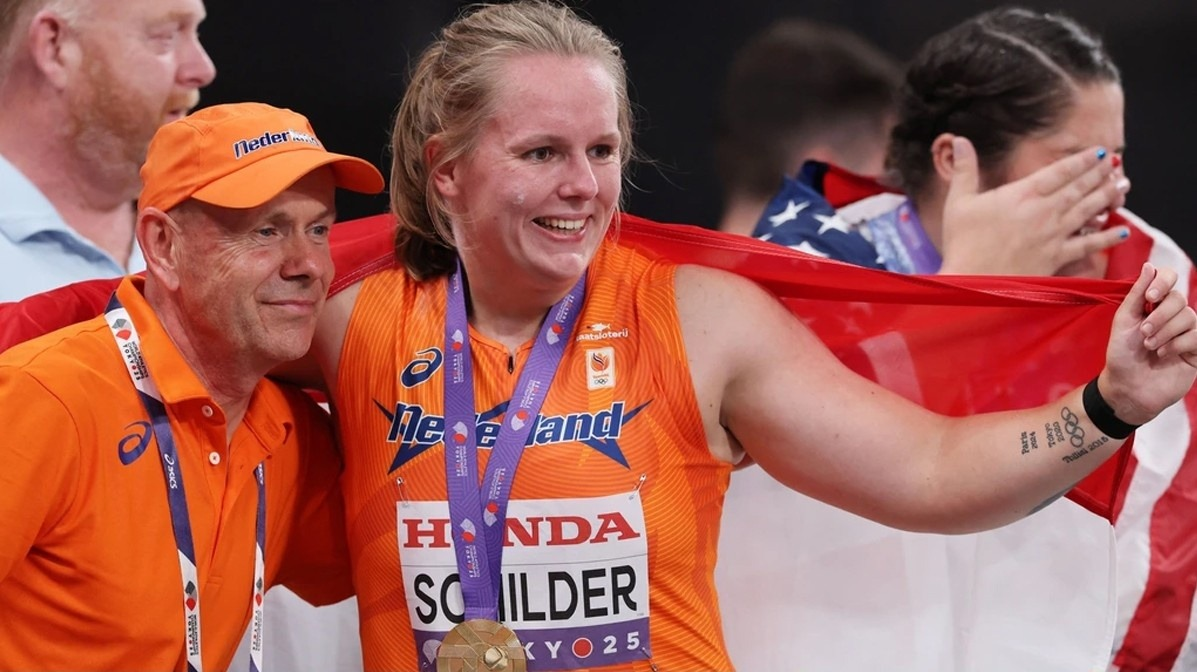
\includegraphics[width=\linewidth]{bilder/sem/strip_a.jpg}\par\vspace{4pt}\noindent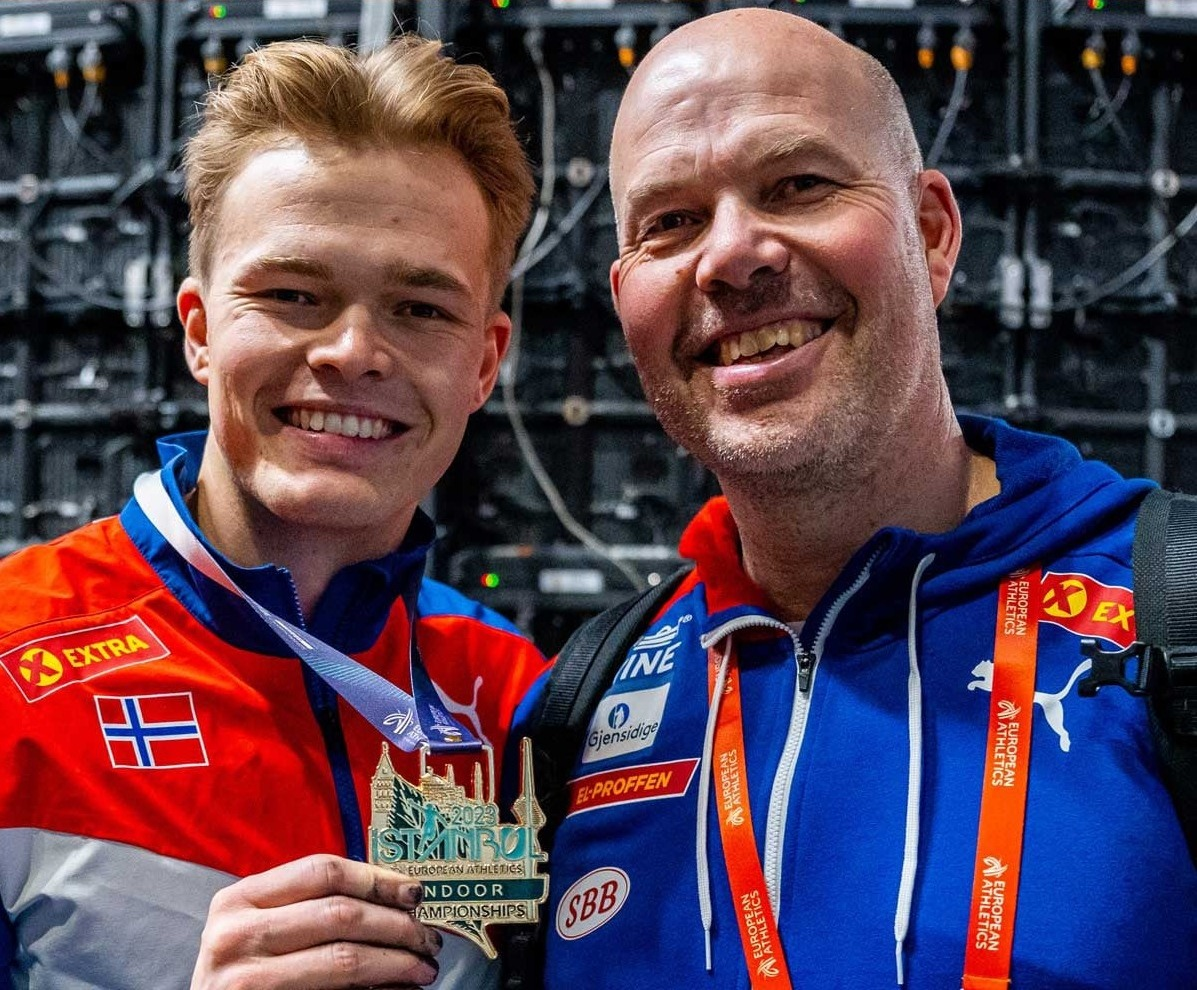
\includegraphics[width=\linewidth]{bilder/sem/strip_b.jpg}\par
\clearpage

% ===== Side 2: fagpersoner =====
\makeatletter
\twocolumn[\begin{@twocolumnfalse}
  \vspace{2mm}
  {\kickfont\small\color{aksent}TRENERSEMINARET 2026\par}\vspace{4pt}
  {\headfont\fontsize{26}{28}\selectfont\color{morkgra}Fagpersonene\par}\vspace{6pt}
  {\noindent\color{aksent}\rule{22mm}{2.4pt}\par}\vspace{10pt}
  \noindent\hbox to \textwidth{\fagperson{im-002.jpg}{Atle Guttormsen}{Stav, bredde og topp}\hfil
  \fagperson{im-003.jpg}{Wolfgang Adler}{Mangekamp, lengde}\hfil
  \fagperson{im-004.jpg}{Gert Damkat}{Kule og diskos}\hfil
  \fagperson{im-005.jpg}{Gina Flugstad Øistuen}{Idrettsfysiolog · REDs}}
  \vskip 6pt
  \noindent\hbox to \textwidth{\fagperson{im-006.jpg}{Jaysuma Saidy Ndure}{Sprint}\hfil
  \fagperson{im-007.jpg}{Vegard Rooth}{Oppvarming for sprint}\hfil
  \fagperson{im-008.jpg}{Mariusz Wo\'zniak}{Mellom- og langdistanse}\hfil
  \fagperson{im-009.jpg}{Bjørn Johansen}{Sprint og spenst}}
  \vspace{8pt}{\noindent\color{lysgra!35}\rule{\textwidth}{0.5pt}\par}\vspace{6pt}
\end{@twocolumnfalse}]
\makeatother
\gdef\toppseksjon{Trenerseminaret}

\bio{Atle Guttormsen}{Atle Guttormsen er først og fremst kjent som far og trener til stavhopperne Sondre og Simen Guttormsen som han har trent til henholdsvis 6,06 meter og 5,80 meter. Utover det har Atle bekledd de fleste roller i norsk friidrett. Han har sittet i styret i NFIF, han har vært kretsleder og klubbleder. Han er bronsedommer og han er godkjent athlete representative (agent). I det sivile er Atle professor i økonomi, men har de siste årene rettet mer og mer av forskningen sin inn mot friidrett.}
\bio{Wolfgang Adler}{Former National Team Coach and Team Leader – Jumps, Austrian Athletics Federation (ÖLV). High Performance Coach at the Austrian High Performance Centre (BLZ) Linz. Currently Coach Developer at Swiss Athletics and Coach at the National High Performance Centre Northwest Switzerland (NLZ, Basel). Has coached athletes across a wide range of disciplines, including medal-winning athletes at international competitions – from Mountain Running to Combined Events.}
\bio{Gert Damkat}{Trener på klubbnivå siden 1984. Landslagstrener for Nederland på deltid fra 2000 og fulltid fra 2006. Har tidligere trent Rutger Smith og Eric Cadée. Er nå personlig trener for regjerende verdensmester i kule Jessica Schilder og diskoskasterne Ruben Rolvink og Shaquille Emanuelson, som begge var finalister i EM i diskos i 2026.}
\bio{Gina Flugstad Øistuen}{Idrettsfysiolog fra Norges idrettshøgskole. Master innen fysisk prestasjonsevne med spesialisering i kvinner og utholdenhetsprestasjon. Personlig trener ved Ambassaden trening, engasjert av NFIF i «Hun satser», og foreleser og fagartikkelforfatter ved Akademiet for Personlig Trening. Aktiv løper med bakgrunn som langrennsløper.}
\bio{Jaysuma Saidy Ndure}{Trener i IL i BUL, der han trener flere av Norges beste sprintere. Han har en lang karriere fra internasjonalt toppnivå og er fortsatt norsk rekordholder på 100 meter med 9,99 og 200 meter med 19,89. Som utøver deltok han i en rekke OL, VM og EM. I trenerrollen bruker han erfaringene fra egen toppidrettskarriere til å utvikle nye norske sprintere på høyt nivå.}
\bio{Vegard Rooth}{Vegard Rooth er friidrettstrener i Lambertseter IF og har blant annet trent datteren Andrea Rooth, som har vunnet U23-EM på 400 meter hekk og U20-EM på samme distanse. Han har selv bakgrunn som friidrettsutøver med flere NM-medaljer, og har også treneroppgaver i Norges Friidrettsforbund. Ved siden av friidretten arbeider han med ledelse og prestasjonsutvikling i næringslivet.}
\bio{Mariusz Wo\'zniak}{Mariusz Wo\'zniak er en polsk friidrettstrener med lang erfaring fra norsk og internasjonal mellom- og langdistanseløping. Han har en bachelorgrad i kroppsøving og idrettsvitenskap og en mastergrad i ledelse. Fra 2015 til 2023 var han trener i SK Vidar i Oslo. Wo\'zniak er personlig trener for 24 år gamle Pernille Karlsen Antonsen, som har en personlig rekord på 1.58,82 på 800 meter. Innendørs satte hun norsk rekord med 2.00,77. Wo\'zniak er nå hovedtrener for utholdenhetsblokken i det polske friidrettsforbundet (PZLA), med overordnet ansvar for mellom- og langdistanseløping. I denne rollen fungerer han som sportslig ansvarlig og koordinator for utøvere og deres personlige trenere, blant andre Klaudia Kazimierska og hennes trener Jerry Schumacher, samt Maciej Wyderka og hans trener Janusz Szczyrek.}
\bio{Bjørn Johansen}{Bjørn Johansen er sprint- og hekktrener i Ranheim IL og Trondheim Friidrett, og fungerer også som kretstrener i Sør-Trøndelag. Han har lang erfaring som trener for utøvere fra ungdomsnivå til senior. Ved siden av trenerarbeidet er han lektor ved Byåsen videregående skole og PhD-kandidat i profesjonsvitenskap ved Nord universitet. PhD-arbeidet hans undersøker sammenhengen mellom horisontale hopp og sprintprestasjon, og hvilken effekt ulike former for hopptrening kan ha på sprint. Han er også mangeårig styremedlem i Trenerforeningen.}

% ===== Side 3: program lørdag =====
\onecolumn\begingroup
\gdef\toppseksjon{Trenerseminaret}
\vspace*{1mm}
{\kickfont\small\color{aksent}PROGRAM\par}\vspace{3pt}
{\headfont\fontsize{26}{28}\selectfont\color{morkgra}Lørdag 21. november\par}\vspace{4pt}
{\noindent\color{aksent}\rule{22mm}{2.4pt}\par}
\linespread{1}\selectfont\renewcommand{\arraystretch}{1.0}\setlength{\tabcolsep}{4pt}
\bolkoverskrift{Felles foredrag}
\noindent\begin{tabular}{@{}p{22mm}p{0.40\textwidth}p{0.40\textwidth}@{}}
\tid{09:15}&\multicolumn{2}{p{0.82\textwidth}}{\foredragstittel{Registrering}\hspace{1em}\foredragsunder{Pausemat tilgjengelig fra kl. 09:00}}\\
\tid{10:00–10:15}&\multicolumn{2}{p{0.82\textwidth}}{\foredragstittel{Velkommen}}\\[1pt]
\tid{10:15–11:00}&\multicolumn{2}{p{0.82\textwidth}}{\foredragsholder{Atle Guttormsen}\quad\foredragstittel{Har bredde noe å si for topp? Har topp noe å si for bredde?}}\\
\pauselinje{11:00–11:15}{Pause}
\tid{11:15–12:00}&\multicolumn{2}{p{0.82\textwidth}}{\foredragsholder{Wolfgang Adler}\quad\foredragstittel{The Long-Term Journey. Coaching, Development \& the Swiss Athletics System}}\\
\pauselinje{12:00–12:15}{Pause}
\tid{12:15–13:00}&\multicolumn{2}{p{0.82\textwidth}}{\foredragsholder{Gina Flugstad Øistuen}\quad\foredragstittel{REDs – når kroppen går i sparemodus: konsekvenser og risikofaktorer}\newline\foredragsunder{Relativ energimangel i idrett (REDs)}}\\
\pauselinje{13:00–14:00}{Lunsj}
\end{tabular}
\bolkoverskrift{Parallelle foredrag}
\noindent\begin{tabular}{@{}p{22mm}p{0.40\textwidth}p{0.40\textwidth}@{}}
\tid{14:00–14:45}&\foredragsholder{Wolfgang Adler}\newline\foredragstittel{The Puzzle of Combined Events. How to Develop, Connect and Balance Performance. Part 1}&\foredragsholder{Mariusz Wo\'zniak}\newline\foredragstittel{Talentutvikling i Norge vs. Polen på mellomdistanse}\\
\pauselinje{14:45–15:00}{Pause med forfriskninger}
\tid{15:00–15:45}&\foredragsholder{Wolfgang Adler}\newline\foredragstittel{The Puzzle of Combined Events. How to Develop, Connect and Balance Performance. Part 2}&\foredragsholder{Gert Damkat}\newline\foredragstittel{Developing the complete thrower}\newline\foredragsunder{Strength, power and movement for shot put and discus}\\
\pauselinje{15:45–16:00}{Pause}
\tid{16:00–17:00}&\foredragsholder{Jaysuma Saidy Ndure}\newline\foredragstittel{Sprinttrening – filosofi, prinsipper og treningsprogram}&\foredragsholder{Gert Damkat}\newline\foredragstittel{Unlocking distance in the rotational shot put}\newline\foredragsunder{Technical principles for better performance}\\
\pauselinje{17:00–17:15}{Pause}
\tid{17:15–18:15}&\foredragsholder{Atle Guttormsen}\newline\foredragstittel{Hva er viktigst i den generelle treningen, og hva er de viktigste tekniske elementene i stav?}\newline\foredragsunder{Hva jeg mener bør være i fokus fra starten av – og «hva vi har gjort».}&\foredragsholder{Mariusz Wo\'zniak}\newline\foredragstittel{Hva skal til for å lykkes på 800 m. Treningsfilosofi og treningsopplegg}\\
\pauselinje{18:15–18:30}{Pause}
\tid{18:30–19:30}&\foredragsholder{Bjørn Johansen}\newline\foredragstittel{Spenst og sprintprestasjon – fra forskning til treningspraksis}\newline\foredragsunder{Erfaringer og funn fra egen PhD om horisontale hopp og sprint}&\foredragsholder{Gert Damkat}\newline\foredragstittel{Mastering discus technique}\newline\foredragsunder{Building efficient and effective throwing mechanics}\\
\end{tabular}
\vspace{8pt}
\begin{tcolorbox}[enhanced,colback=hovedbla,colframe=hovedbla,arc=0pt,boxrule=0pt,left=10pt,right=10pt,top=6pt,bottom=6pt]
\tid{\color{white}20:00}\hspace{1.2em}{\sffamily\bfseries\color{white}Middag}\hspace{0.8em}{\sffamily\small\color{white}3-retters middag med utdeling av prisen Årets trener.}
\end{tcolorbox}
\clearpage

% ===== Side 4: søndag, priser, påmelding =====
\gdef\toppseksjon{Trenerseminaret}
\vspace*{1mm}
{\kickfont\small\color{aksent}PROGRAM\par}\vspace{3pt}
{\headfont\fontsize{26}{28}\selectfont\color{morkgra}Søndag 22. november\par}\vspace{4pt}
{\noindent\color{aksent}\rule{22mm}{2.4pt}\par}\vspace{2pt}
\linespread{1}\selectfont\renewcommand{\arraystretch}{1.0}\setlength{\tabcolsep}{4pt}
\noindent\begin{tabular}{@{}p{22mm}p{0.40\textwidth}p{0.40\textwidth}@{}}
\tid{09:00–09:30}&\multicolumn{2}{p{0.82\textwidth}}{\foredragstittel{Årsmøte Trenerforeningen}}\\[1pt]
\tid{10:00}&\multicolumn{2}{p{0.82\textwidth}}{\foredragstittel{Buss til Nes Arena}\hspace{1em}\foredragsunder{Praktiske økter}}\\[1pt]
\tid{10:30–11:30}&\foredragsholder{Gert Damkat}\newline\foredragstittel{Around and inside the shot put circle}\newline\foredragsunder{Live coaching and technical problem solving}&\foredragsholder{Jaysuma Saidy Ndure}\newline\foredragstittel{Sprinttrening i praksis med Jaysuma Saidy Ndure}\\
\pauselinje{11:30–11:45}{Pause}
\tid{11:45–12:45}&\multicolumn{2}{p{0.82\textwidth}}{\foredragsholder{Wolfgang Adler}\newline\foredragstittel{Long Jump – From the Central Sequence to Combined Events}}\\
\pauselinje{12:45–13:00}{Pause}
\tid{13:00–14:00}&\foredragsholder{Gert Damkat}\newline\foredragstittel{Around and inside the discus circle}\newline\foredragsunder{Live coaching and technical problem solving}&\foredragsholder{Vegard Rooth og Andrea Rooth}\newline\foredragstittel{God oppvarming, den viktigste treningen?}\\
\tid{14:00}&\multicolumn{2}{p{0.82\textwidth}}{\foredragstittel{Lunsj i Nes Arena}}\\
\tid{14:50}&\multicolumn{2}{p{0.82\textwidth}}{\foredragstittel{Buss til Gardermoen fra Nes Arena}\hspace{1em}\foredragsunder{Rutebuss}}\\
\end{tabular}

\vspace{14pt}
{\kickfont\small\color{aksent}PRISER OG PÅMELDING\par}\vspace{3pt}
{\noindent\color{aksent}\rule{22mm}{2.4pt}\par}\vspace{8pt}
\label{sem:pris}
\begin{tcolorbox}[enhanced,colback=bakgrunn,colframe=bakgrunn,arc=0pt,boxrule=0pt,left=12pt,right=12pt,top=8pt,bottom=8pt]
\sffamily\small\renewcommand{\arraystretch}{1.5}
\begin{tabular*}{\linewidth}{@{\extracolsep{\fill}}lr@{}}
Fullt seminar & \textbf{2\,600 kr}\\
Fullt seminar – medlem Trenerforeningen & \textbf{2\,400 kr}\\
Fullt seminar – ungdom (født fra 2001) & \textbf{2\,400 kr}\\
Seminar kun lørdag & \textbf{2\,000 kr}\\
Seminar kun søndag & \textbf{1\,000 kr}\\
Middag lørdag – 3-retters & \textbf{695 kr}\\
\end{tabular*}
\end{tcolorbox}
\vspace{8pt}
\begin{tcolorbox}[enhanced,colback=aksent,colframe=aksent,arc=0pt,boxrule=0pt,left=14pt,right=14pt,top=10pt,bottom=10pt]
{\kickfont\large\color{white}PÅMELDINGSFRIST: 9. NOVEMBER 2026}\\[1pt]{\sffamily\small\color{white}Meld deg på Trenerseminaret 2026 via Trenerforeningen.}
\end{tcolorbox}
\clearpage
\endgroup\twocolumn

\end{document}
